
The approaches presented herein are inspired by \cite{mcnotes}.



Let $\chain$ be the chain under consideration, $X_i \sim \dist$ with $\dist$ some distribution and $\phi : \R \rightarrow \R$ be a function. 

$\phi$ is used to estimate key quantities describing $\dist$ by evaluating $\int \phi(x) \, dP(x)$; setting $\phi = id$ yields the mean and $\phi(x) := x^2$ yields the variance (assuming the chain has mean $0$).

 
With this setup, there are several aspects of convergence to consider: 
\begin{itemize}
	\item whether the chain has reached a stationary regime
	\item whether the chain explores the full support of the target distribution 
	\item the independence of the chain's elements 
\end{itemize}

In the following, we will not address the second aspect. This is because the distribution we are sampling from is a posterior distribution, whose closed form is unavailable to us. Hence, there is no straightforward way to define the support we expect the distribution to have.

\subsection{Stationarity}
Let 
\[
	\edf{x} := \frac{\sum_{i=1}^T 1_{X_i \leq x}}{T}
\]
This is called the \textit{empirical distribution function}. One can show that the empirical distribution function converges almost surely towards the distribution function for any $x \in \R$. 

Once the chain has reached its stationary regime, we expect the empirical distribution function to have almost converged as well. We adopt an idea originally presented by Dr. Pieralberto Guarniero in a practical seminar in the context of Riemann sums: 
The chain of length $T$ is split into three components of equal size $s := \floor{\frac{T}{3}}$: 
\[
S_1 := \left(X_1, \dots, X_s\right), S_2 := \left(X_s, \dots, X_{2s}\right), S_3 := \left(X_{2s}, \dots, X_T\right)
\] 

Figure \ref{splitChain} illustrates how the chain is split. Note that in the first part, the parameters are still diverging from their initial values; this part is referred to as  ''burn-in period''. Note that because the way from the initial estimates is included, this part's empirical distribution function is usually far from the desired distribution. Therefore, the very first part is usually ignored in this analysis.

Upon a brief, graphical inspection, one might conclude that the second and third part's distribution seems to be equal and in particular, that the distribution reached stationarity after about $50$ samples.  


Figure \ref{splitChainDensities} shows the estimates densities (as they are graphically easier to understand than the estimated empirical distribution function itself) for all three parts of the chain; one can clearly see that the second and third chains' modes are already ''zeroing in'' on the original probability (which is $0.9$, while the first density is still highly skewed towards the initial choice. 

Note how the second chain's density still exhibits multiple modes, whereas the third chain only has one main mode left (which is incidentally closer to the original value). Visual inspection fails to reveal this. However, the median (indicated by a green line) is the same for the second and third part. 


\begin{figure}
	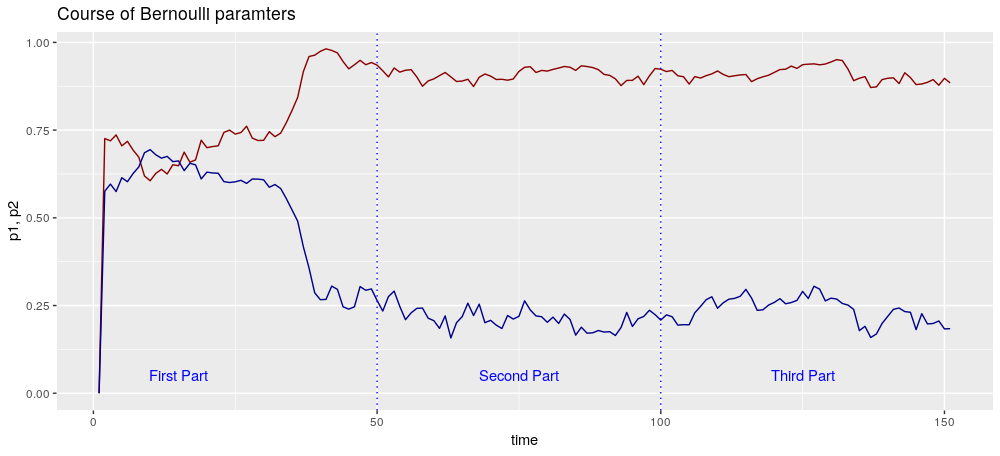
\includegraphics[width=\linewidth]{Images/bernoulli_param_split.png}
	\caption{Course of Bernoulli parameters for Gibb's sampler on simple rain model}
	\label{splitChain}
\end{figure}

\begin{figure}
	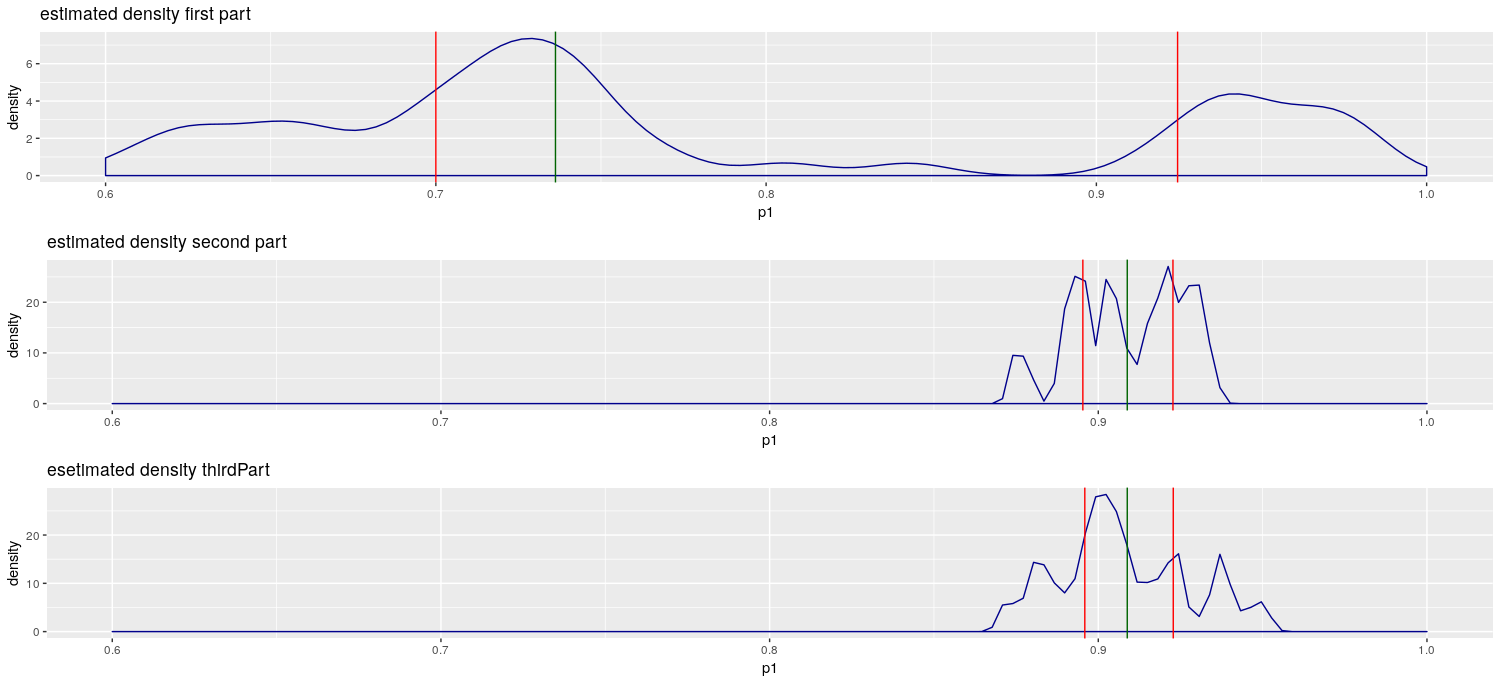
\includegraphics[width=\linewidth]{Images/chain_parts_quantiles.png}
	\caption{Density estimates for $S_1, S_2$ and $S_3$ with $0.25, 0.5$ and $ 0.75$ quantiles (red, green, red) indicated by lines}
	\label{splitChainDensities}
\end{figure}

Figure \ref{splitChainQuantileCourse} allows us to quantitatively confirm the results from the visual inspection. We observe:
\begin{itemize}
	\item the third part reaches its stationary regime earlier than the second part
	\item the second part's quantiles converge toward the third part's quantiles
\end{itemize}

Note that the second and third parts' quantiles in figure \ref{splitChainQuantileCourse} become visually indistinguishable after a sample size of about $120$. 

At this point, the maximum difference has fallen below $0.01 (1\%)$. 
Also, the second part comprises elements from about $X_{40}, \dots, X_{80}$ whereas the third part comprises $X_{80}, \dots, X_{120}$. This is consistent with our intuitive conclusion from figure \ref{splitChain} that the chain reaches its stationary regime after about $50$ samples. 

\begin{figure}
	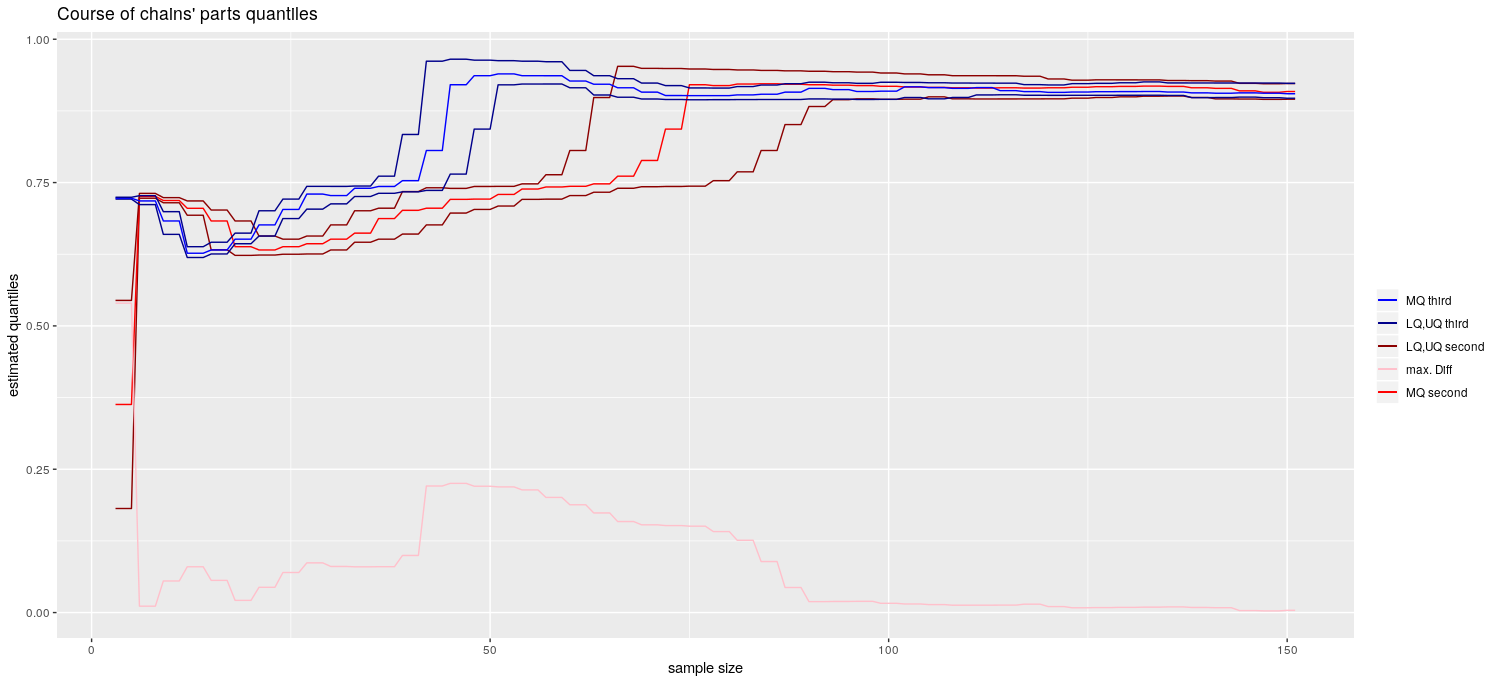
\includegraphics[width=\linewidth]{Images/chain_part_quantiles.png}
	\caption{Course of Quantiles for the second and third part of the chain. ''LQ, MQ and UP'' are shortcuts for ''lower'', ''middle'' and ''upper' quantile and refer to the $0.25, 0.5$ and $0.75$ quantiles, respectively. ''second'' and ''third' refer to which part of the chain is considered for computing the quantiles. ''Max. Diff'' (pink) denotes the maximum difference between respective quantiles at each point in time. }
	\label{splitChainQuantileCourse}
\end{figure}

We shall adopt the criterion developed herein with a cut-off criterion of $0.01$. That is to say: 

\begin{center}
We assume that the chain has reached convergence once the maximum difference between the $0.25, 0.5$ and $0.75$ quartiles of the second and third part are below $0.01$. 
\end{center}

\subsection{Independence of Elements}

